\documentclass[]{article}
\usepackage{amssymb}
\usepackage{amsmath}
\usepackage[utf8]{inputenc}
\usepackage{graphicx}
\usepackage{booktabs}
\usepackage{listings}
\usepackage{color}
\usepackage{tabularx}
\usepackage{hyperref}

\definecolor{dkgreen}{rgb}{0,0.6,0}
\definecolor{gray}{rgb}{0.5,0.5,0.5}
\definecolor{mauve}{rgb}{0.58,0,0.82}

\lstset{frame=tb,
	%language=C++,
	aboveskip=3mm,
	belowskip=3mm,
	showstringspaces=false,
	columns=flexible,
	basicstyle={\small\ttfamily},
	numbers=none,
	numberstyle=\tiny\color{gray},
	keywordstyle=\color{blue},
	commentstyle=\color{dkgreen},
	stringstyle=\color{mauve},
	breaklines=false,
	breakatwhitespace=true,
	tabsize=2
}


\title{FYS-STK4155 H20 - Project 3:\\Time Series Analysis with AR and RNN Models}
\author{Olav Fønstelien}

\begin{document}
\maketitle

\begin{abstract}
%The abstract gives the reader a quick overview of what has been done and the most important results. Try to be to the point and state your main findings. It could be structured as follows 
% - Short introduction to topic and why its important 
% - Introduce a challenge or unresolved issue with the topic (that you will try to solve) 
% - What have you done to solve this 
% - Main Results 
% - The implications

\end{abstract}

\section{Introduction} \label{sec:intro}
%When you write the introduction you could focus on the following aspects
% - Motivate the reader, the first part of the introduction gives always a motivation and tries to give the overarching ideas
% - What I have done
% - The structure of the report, how it is organized etc

% intro to condition monitoring of electric machines
% intro to insulation and temperature
% intro to transformers

Electric machines are highly reliable when properly designed and maintained. They are the workhorses in any industrial process, as well as the actuator in safety-critical functions, and failure may have both economic and physical consequences in the form of downtime and personnel injury. Ensuring proper function of the machinery is a major cost driver in industry -- dedicated technicians are employed to execute detailed maintenance schedules while others log and monitor performance indicators like temperature and vibration. Improving and automating such procedures is a large part of what \textit{Industry 4.0} is about. \textit{Digital twins} of the machines can be used to predict faults which are developing too slowly to be noticed, or which may not even be detectable with regular instrumentation. 

Machine learning methods play a vital part in developing digital twins and in this report we will see how a simple model for condition monitoring of the cooling efficiency of an electric power transformer can be created by the use of traditional autoregression (AR) and neural networks. Even small increases in a transformer's operating temperature may have severe effects on the lifetime of its electrical insulation, and ensuring that the cooling system performs as designed is vital for reliability and performance of the transformer. We will create model of the transformer which lets us evaluate the cooling system's performance under dynamic operating conditions based only on a few input measurements which are normally monitored in a standard plant automation and control system. The performance at the time of model creation will serve as the baseline against which future performance will be measured.


Structure of report [....], but first a short review of the basics of power transformers.



\subsection{Electric Power Transformer Basics} \label{sec:transformers}
Electrical power distribution networks usually have several voltage levels, and its the power transformer's job to \textit{transform} the power from one voltage level to another. In a three-phase power system, each phase will be connected to separate transformer \textit{windings} -- one per phase for the high voltage (HV) side and one for the low voltage (LV) side. The HV and LV windings of each phase are usually installed like concentric cylinders with the ferromagnetic core in the middle for magnetic coupling between them. The phase windings are physically separated from each other, but they are usually installed together either inside a tank containing cooling oil, or an air-filled enclosure, like the one we will treat in this report. 

A typical example is shown in Figure \ref{fig:dry-transformer}. The three phase windings, denoted $U, V, W$, are the red barrel-like structures seen inside the (opened) enclosure. The windings, usually made of copper or aluminium, develop heat when they conduct current. The phase windings are therefore constructed with a gap between the concentric HV and LV winding to allow air to flow between them for cooling. During operation the transformer is fully enclosed and air is circulated by the cooling fan motors, which we see on the outer wall to the upper left (blue-gray). The air is forced through the windings by the horizontal separation plate at the bottom of the windings. The heat dissipated by the windings is drawn out of the system by an air-water heat exchanger, which is located below the motors close to the floor. 

The winding insulation on this type of air-cooled transformers is usually made of epoxy, which is mechanically robust and has good electric insulating properties. Epoxy consists of long hydrocarbon chains which has a temperature-dependent degradation rate, such that a 6 kelvin increase in temperature approximately halves the useful lifetime of the material (\textit{Arrhenius' law}). Expected lifetime under nominal operating conditions is 180.000 hours ($\sim 20$ years), which will of course vary greatly between manufacturers and even otherwise identical units from the same manufacturer \cite{iec60076-12}.

The operation of the transformer is monitored by reading phase currents and winding temperatures, as well as the operational status of auxiliary systems like cooling fans. The measurements are transmitted to the plant automation and control system which monitors the condition of the transformer together with other equipment in the plant, and which may also store measurements digitally on a server. See \cite{hubert2002} for an easy-to-read introduction to electric machines.

\begin{figure}[!h]
	\centering
	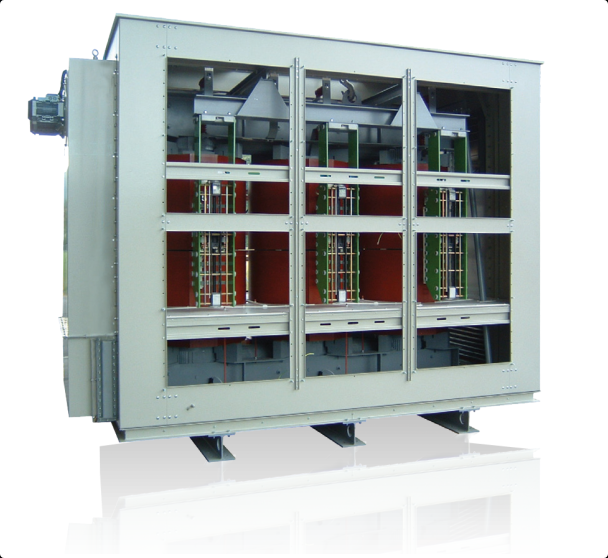
\includegraphics[width=1\linewidth]{./figs/dry-transformer.png}
	\caption{Typical air-cooled transformer with three phases $U, V, W$. The windings are the red barrel-like structures seen inside the cabinet, and the HV winding is placed within the LV winding as two concentric cylinders wrapped around the ferromagnetic core. Note that the transformer seen here is for illustrative purposes only and does not relate to the results in this report in any way.}
	\label{fig:dry-transformer}
\end{figure}


\section{Methods} \label{sec:methods}
% - Describe the methods and algorithms
% - You need to explain how you implemented the methods and also say something about the structure of your algorithm and present some parts of your code
% - You should plug in some calculations to demonstrate your code, such as selected runs used to validate and verify your results. The latter is extremely important!! A reader needs to understand that your code reproduces selected benchmarks and reproduces previous results, either numerical and/or well-known closed form expressions.

For the design, training and testing of our transformer temperature model, we have a dataset provided by ABB AS \cite{abb-url}. The dataset contains operational data from a 12 MVA (mega volt-amperes) transformer as a time series stretching over approximately 14 months. Sampling rates are between 1 second and 1 minute, depending on the signal.

Failure or degradation of the transformer cooling system may take one of two forms -- either as an overall problem, which will present itself as increased operation temperature of the whole transformer; or as a failure affecting only one transformer phase winding, giving increased temperature in that winding. 

Common causes for the first would be reduced air flow due to a damaged impeller or oxidation inside the heat exchanger, which will reduce its efficiency. Especially oxidation is a slowly-developing fault which may be difficult to spot. To discover such developments, we need a fine-tuned model which precisely predicts the winding temperature in a healthy transformer in any operation condition. Deviation in actual temperature from the predicted temperature will then be indicative of a fault. For this \textit{overall temperature model}, phase current and the running status of the cooling fans will be our input. The temperature of the water flowing into the heat exchanger as well as the room temperature would of course be highly valuable as well, but those measurements are not available in the data which we have.

The other type of fault, affecting only one of the three transformer windings, would typically be caused by mechanical obstruction of the air flow through the winding, for instance by an air guide which has come loose. For this \textit{relative temperature model}, the temperature of the other windings will be the most important input, since they will be mostly unaffected by this. Again, deviation from the predicted temperature will be indicative of failure.

In the following, we will explore three different approaches for creating these models; first a physical model approach where we use what we know about heat dissipation in electrical conductors along with \textit{Newton's law of cooling}; then a traditional autoregressive (AR) model approach, which will yield an equation which can easily be solved by the Ordinary Least Squares (OLS) method; and lastly by using a recursive neural network (RNN) model, suitable for time series data.

\subsection{First Approach: Physical Models} \label{sec:physical-model}

The efficiency of air-cooled transformers usually lay in the 98-99 \% range. For the transformer studied here, that translates to some 120-240 MW. Most of the losses are due to electrical resistance in the windings and are dissipated as heat, which must be transported out through the cooling system. The resistance is temperature dependent, and within normal operating temperatures the heat dissipation at temperature $T$ is given by
\begin{equation}
	\dot{Q}_T = I^2 [R + \alpha(T - T_0)],
\end{equation}
where $I$ is the phase current, $R$ is the resistance at reference temperature $T_0$ (usually 20 $^\circ$C) and $\alpha$ is the temperature coefficient for the material, which is $\sim 4 \cdot 10^{-3}$ $^\circ \text{C}^{-1}$ for copper and aluminium. 

\subsubsection{Physical Overall Temperature Model} \label{sec:physical-model-overall}

Heat is removed from the transformer through the heat exchanger according to Newton's law of cooling;
\begin{equation}
	\dot{Q}_W = K_W(T - T_W),
\end{equation}
where $T_W$ is the water temperature, and $K_W$ is some constant representing the efficiency of heat transfer from the winding, through the air and out of the heat exchanger. Heat is also removed through the walls of the transformer into the room;
\begin{equation}
	\dot{Q}_A = K_A(T - T_A),
\end{equation}
where $K_A$ is similar to $K_W$, and $T_A$ is the ambient temperature. Heat transfer from the windings to the heat exchanger and the room happens at a delay, since heat is also stored in the system. If we let the total heat capacity of the transformer be $C$, the stored heat at temperature $T$ is given by $Q_S = CT$, such that the heat flow from the windings and out of the transformer is given by the power balance
\begin{equation} \label{eq:heat-flow-compact}
	\dot{Q}_T = C \dot{T} + \dot{Q}_W + \dot{Q}_A.
\end{equation}
Since we are dealing with time series here, it is natural to approximate $\dot{T}$ by its Taylor expansion $\dot{T}_{(t)} = (T_{(t)} - T_{(t-\Delta t)})/ \Delta t$. At time $t$, Equation (\ref{eq:heat-flow-compact}) solved for temperature $T_{(t)}$ then becomes
\begin{equation} \label{eq:heat-flow-expanded-t}
	T_{(t)} = \frac{\frac{C}{\Delta t} T_{(t-\Delta t)} + K_W T_W + K_A T_A + I^2 (R - \alpha T_0)}{\frac{C}{\Delta t} + K_W + K_A - I^2 \alpha}.
\end{equation}

At this point it is tempting to let the resistance temperature coefficient $\alpha = 0$, but normal operating temperature range for a transformer is 30-130 $^\circ$C, meaning that the resistive loss in the windings will vary by $\sim 100 \cdot 4 \cdot 10^{-3} = 40 $ \%, and any accurate model would have to account for this. Further, since we do not know $T_W$ and $T_A$, neither at $t = 0$ nor later, we could maybe assume that they could be held constant. This assumption, however, is likely to not be correct, since the heat from the transformer probably will increase the room temperature and the incoming water temperature, which runs in a closed circuit. In addition, in order to solve this model with traditional methods like the Ordinary Least Squares method, we would have to linearize it, which is not entirely straight-forward. We will therefore abandon this model, but the insights gained here will be useful when we design the features for our autoregressive and our neural network models.

\subsubsection{Physical Relative Temperature Model} \label{sec:physical-model-relative}
In a healthy transformer, the temperature in any of the three windings will be closely linked to the temperature of the two others. Since the the electric impedance must be equal between the windings in order to maintain a balanced system voltage, it is natural to assume that the electric losses will also largely be equally distributed. Any difference in temperature

It is natural to assume a linear relationship between the temperatures


\subsection{Second Approach: An Autoregressive Model} \label{sec:autoregressive-model}

\subsection{Third Approach: A Neural Network Model} \label{sec:neural-model}

\subsection{Data Preparation} \label{sec:data-prep}



\subsection{Subsection} \label{sec:subsection-name}
% The first part deals with structuring and reading the data, much along the same lines as done in projects 1 and 2. Explain how the data are produced and place them in a proper context. 




% You need to include at least two central algorithms, or as an alternative explore methods from decisions tree to bagging, random forests and boosting. Explain the basics of the methods you have chosen to work with. This would be your theory part. 

% Then describe your algorithm and its implementation and tests you have performed. 







\section{Results} \label{sec:results}
% - Present your results
% - Give a critical discussion of your work and place it in the correct context.
% - Relate your work to other calculations/studies
% - An eventual reader should be able to reproduce your calculations if she/he wants to do so. All input variables should be properly explained.
% - Make sure that figures and tables should contain enough information in their captions, axis labels etc so that an eventual reader can gain a first impression of your work by studying figures and tables only.

% Then presents your results and findings, link with existing literature and more. 

\section{Discussion and Conclusion} \label{sec:conclusion}
% - State your main findings and interpretations
% - Try as far as possible to present perspectives for future work
% - Try to discuss the pros and cons of the methods and possible improvements

% Finally, here you should present a critical assessment of the methods you have studied and link your results with the existing literature. 

validation of model by lab tests

may still fail even if perfectly maintained and monitored - ref bathtub curve

\clearpage
\vspace{5mm}

%\clearpage
\bibliographystyle{unsrt}
\bibliography{project3.bib}
\end{document}
